\section{Appendix \label{sec:app}}
The figures related to the report are displayed here.

% COARSE GRAINING METRICS EVOLUTION
\begin{figure}[h]
    \centering
    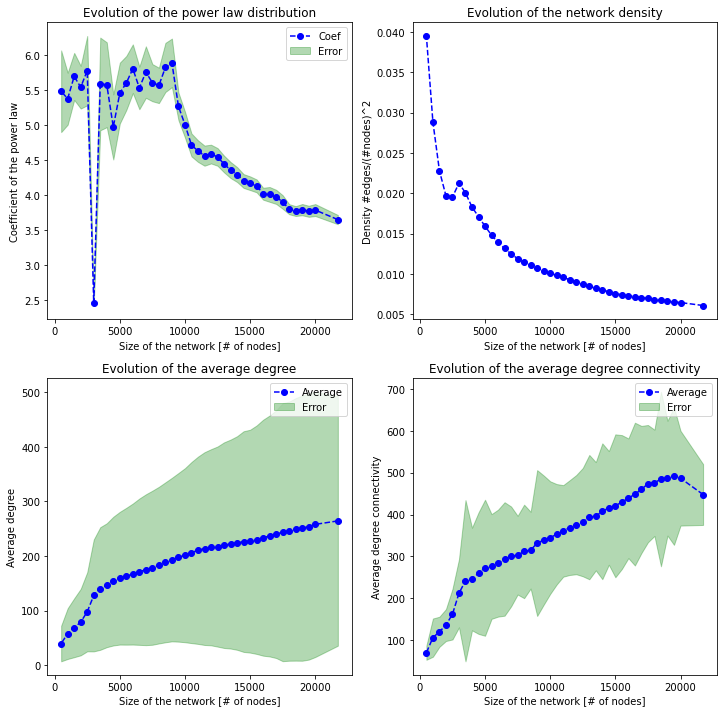
\includegraphics[width=\textwidth]{Images/Coarse/Evolution_graph_coearse.png}
    \caption{Evolution of different metrics along the coarse graining procedure.
    We notice an outlier at $3000$ neurons, that we will analyze in details. We understand
    the various metrics does not change too much up to $10000$ neurons, which is half 
    of the system.}
    \label{fig:coarse_evol}
\end{figure}

% OUTLIER DISTRIBUTIONS
\begin{figure}
    \centering
    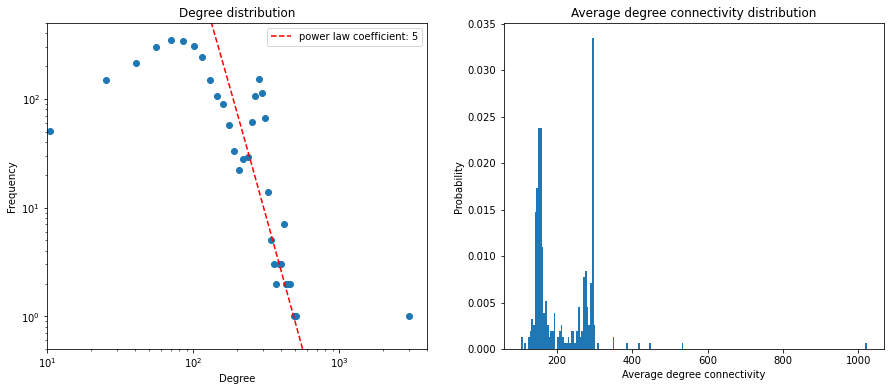
\includegraphics[width=\textwidth]{Images/Coarse/Outlier_distribution.png}
    \caption{Degree and degree connectivity distribution for the outlier point at $N'=3000$ neurons.}
    \label{fig:n3000}
\end{figure}

% DEGREE CONNECTIVITY DISTRIBUTION
\begin{figure}
    \centering
    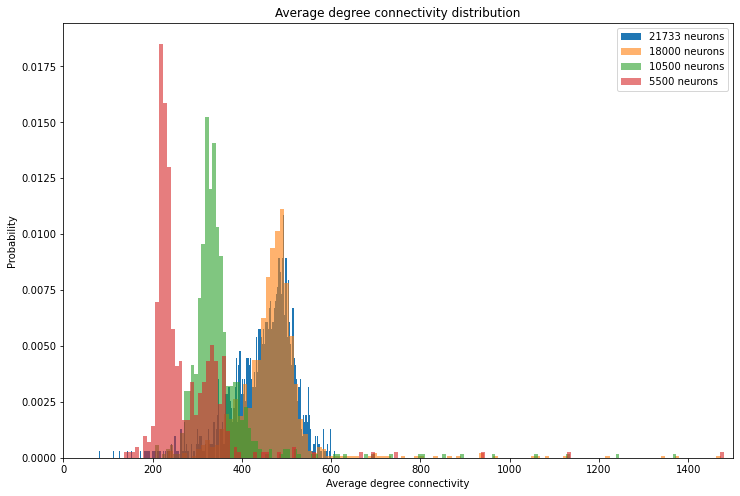
\includegraphics[width=\textwidth]{Images/Coarse/Avg_deg_con_distr.png}
    \caption{Average degree connectivity distribution for different number of neurons along
	the clustering coarse graining technique. We can see both the bi-modality and the presence of 
	super-hubs, as described in the text.}
    \label{fig:con_distr}
\end{figure}

% RANDOM ATTACK
\begin{figure}
	\centering
	\begin{subfigure}[b]{0.45\textwidth}
		\centering
		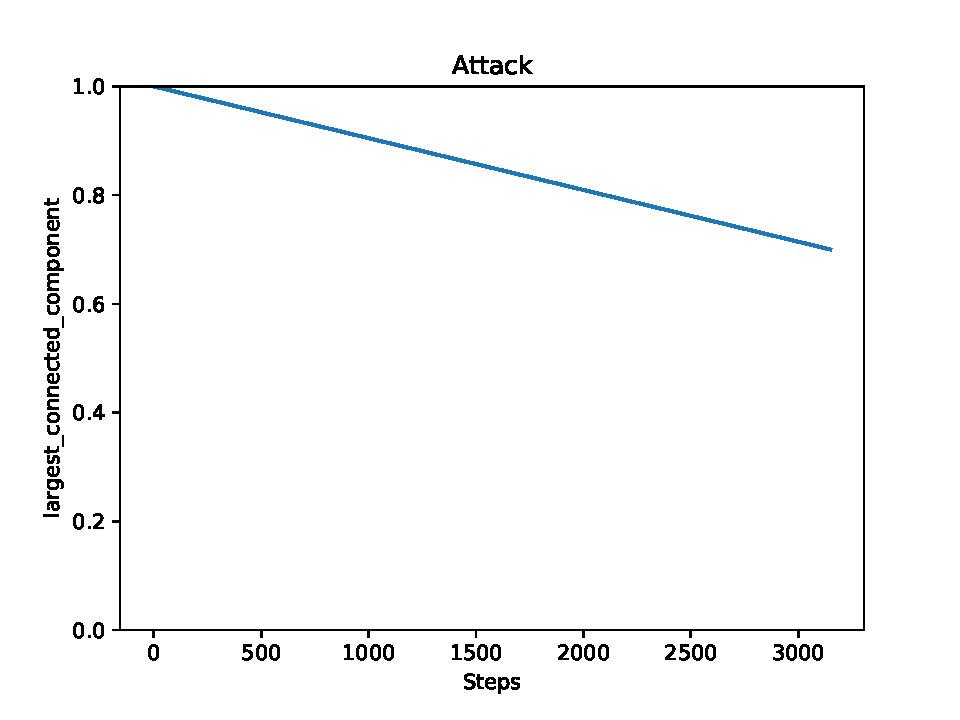
\includegraphics[width=\textwidth]{Images/plots_rnd/rnd_20.pdf}
		\caption{for $10500$ neurons}
		%\label{fig:y equals x}
	\end{subfigure}
	\hfill
	\begin{subfigure}[b]{0.45\textwidth}
		\centering
		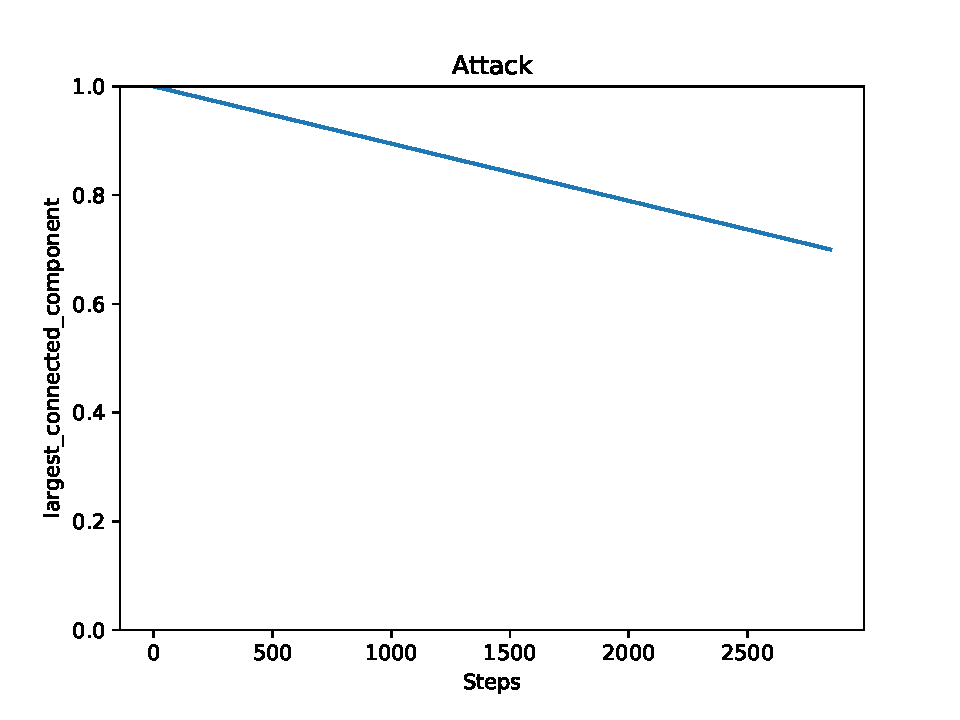
\includegraphics[width=\textwidth]{Images/plots_rnd/rnd_22.pdf}
		\caption{for $9500$ neurons}
		%\label{fig:three sin x}
	\end{subfigure}
	\\ \vspace{5mm}
	\begin{subfigure}[b]{0.45\textwidth}
		\centering
		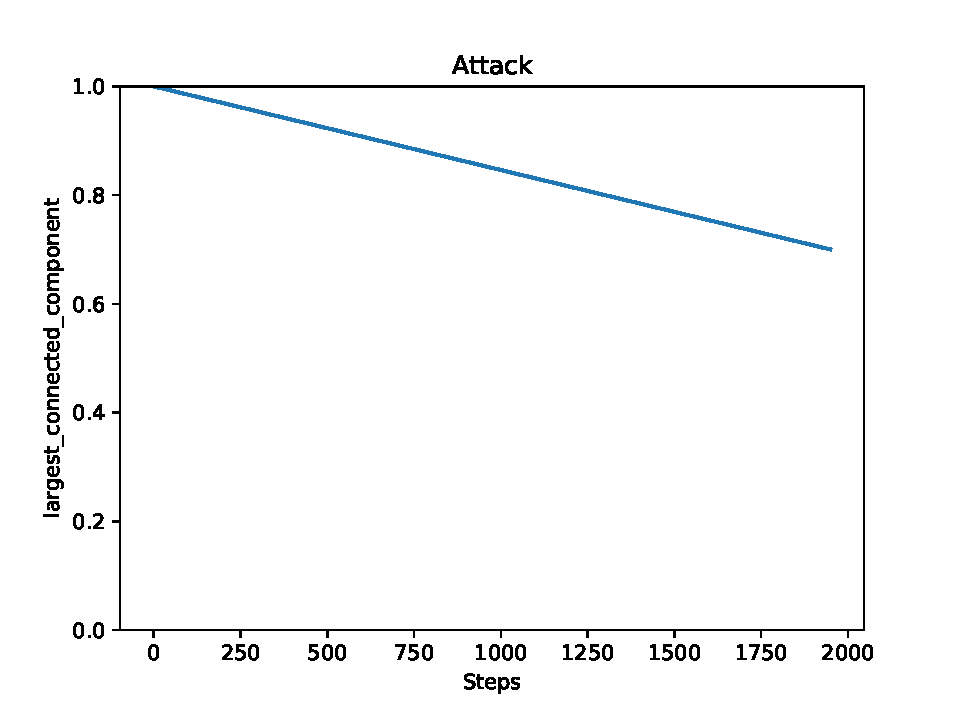
\includegraphics[width=\textwidth]{Images/plots_rnd/rnd_28.pdf}
		\caption{for $6500$ neurons}
		%\label{fig:y equals x}
	\end{subfigure}
	\hfill
	\begin{subfigure}[b]{0.45\textwidth}
		\centering
		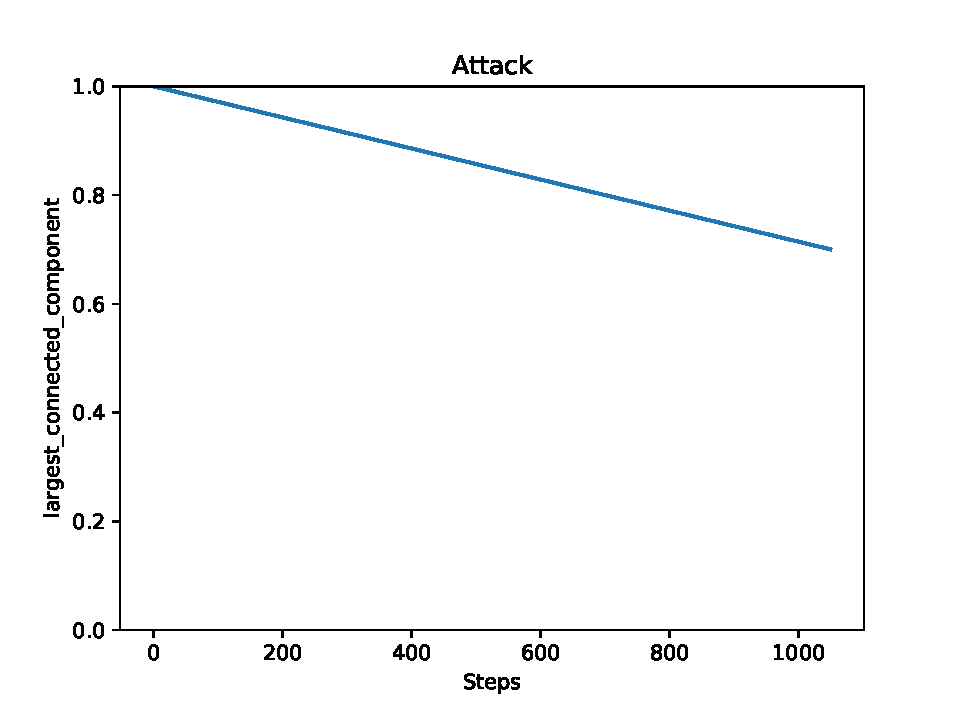
\includegraphics[width=\textwidth]{Images/plots_rnd/rnd_34.pdf}
		\caption{for $3500$ neurons}
		%\label{fig:three sin x}
	\end{subfigure}
	\\ \vspace{5mm}
	\begin{subfigure}[b]{0.45\textwidth}
		\centering
		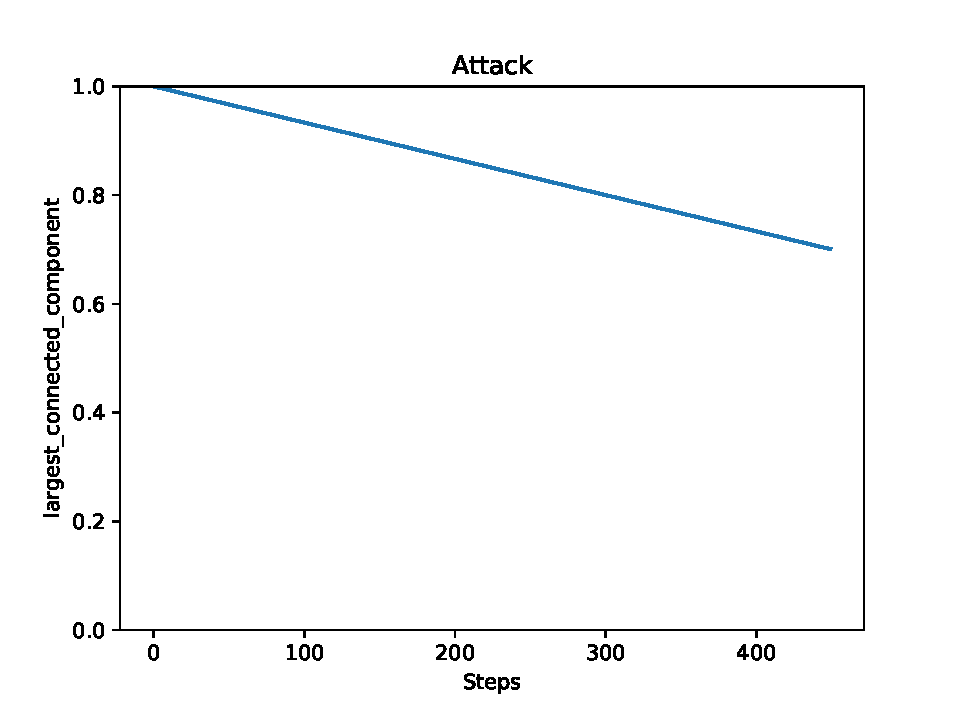
\includegraphics[width=\textwidth]{Images/plots_rnd/rnd_38.pdf}
		\caption{for $1500$ neurons}
		%\label{fig:y equals x}
	\end{subfigure}
	\hfill
	\begin{subfigure}[b]{0.45\textwidth}
		\centering
		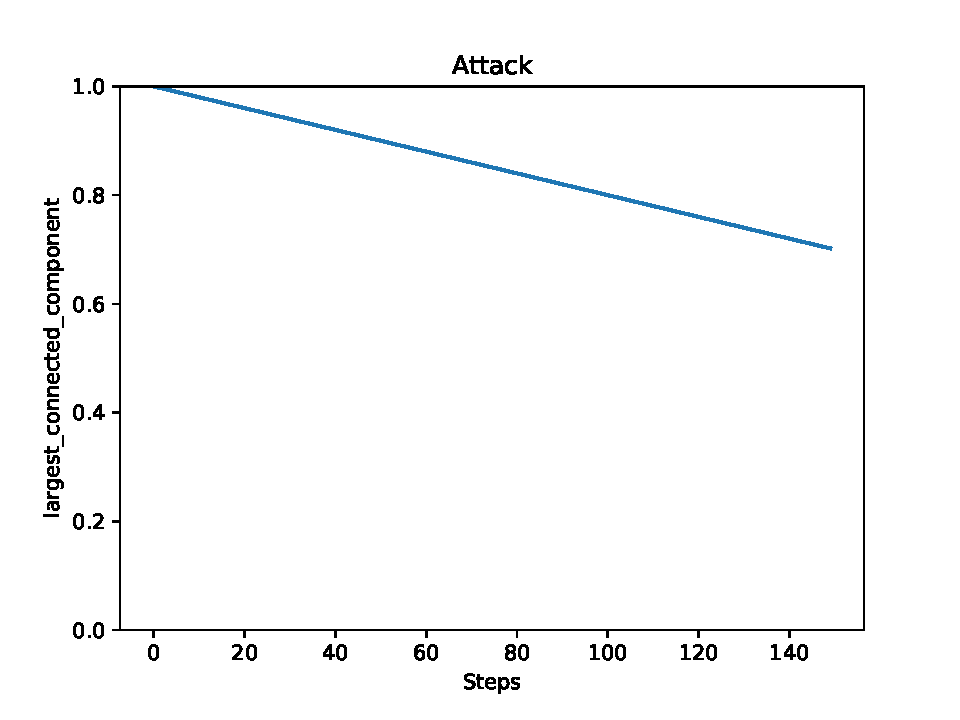
\includegraphics[width=\textwidth]{Images/plots_rnd/rnd_40.pdf}
		\caption{for $500$ neurons}
		%\label{fig:three sin x}
	\end{subfigure}
	\\ \vspace{5mm}
	

	\caption{Robustness of the network at various graining scales against random node removal attacks, using the largest connected component as measure.}
	\label{fig:rnd_atk}
\end{figure}


% BETWEENNESS ATTACK
\begin{figure}
	\centering
	\begin{subfigure}[b]{0.45\textwidth}
		\centering
		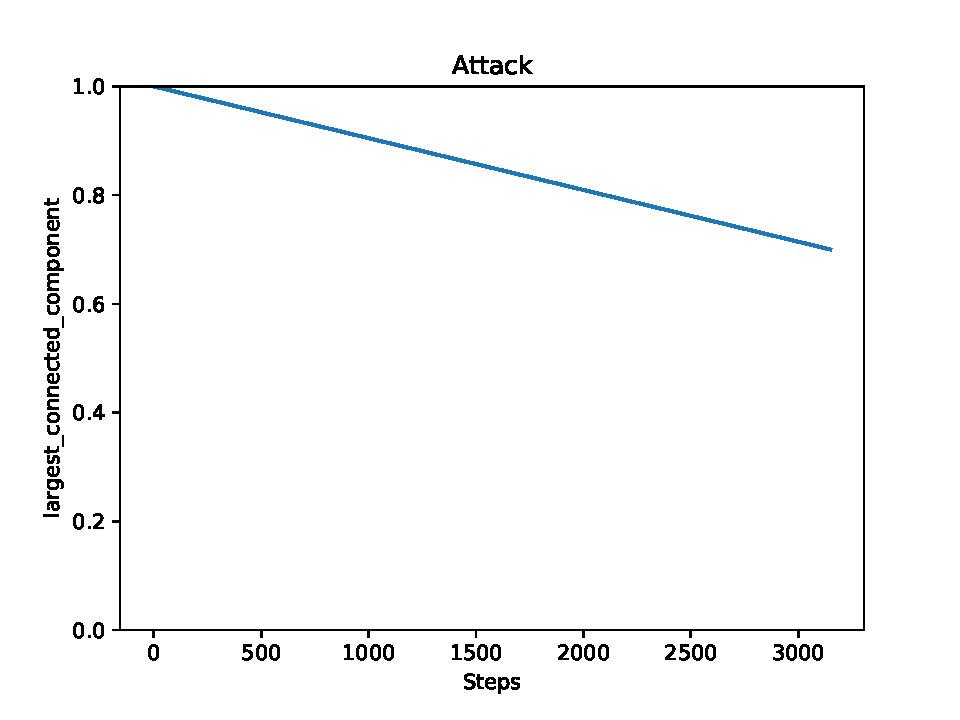
\includegraphics[width=\textwidth]{Images/plots_ib/ib_20.pdf}
		\caption{for $10500$ neurons}
		%\label{fig:y equals x}
	\end{subfigure}
	\hfill
	\begin{subfigure}[b]{0.45\textwidth}
		\centering
		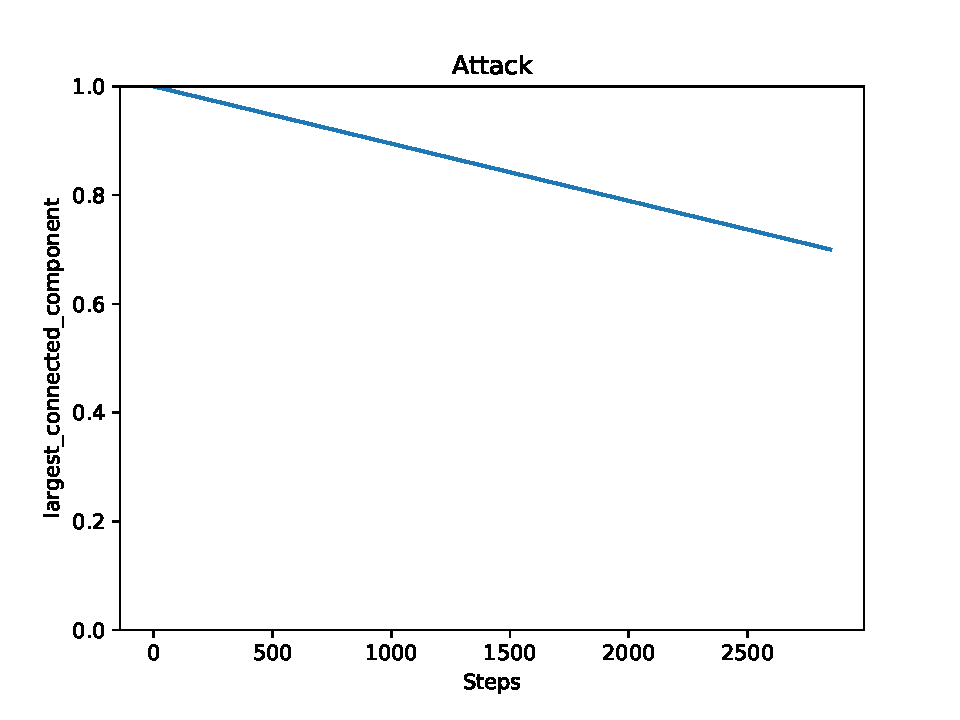
\includegraphics[width=\textwidth]{Images/plots_ib/ib_22.pdf}
		\caption{for $9500$ neurons}
		%\label{fig:three sin x}
	\end{subfigure}
	\\ \vspace{5mm}
	\begin{subfigure}[b]{0.45\textwidth}
		\centering
		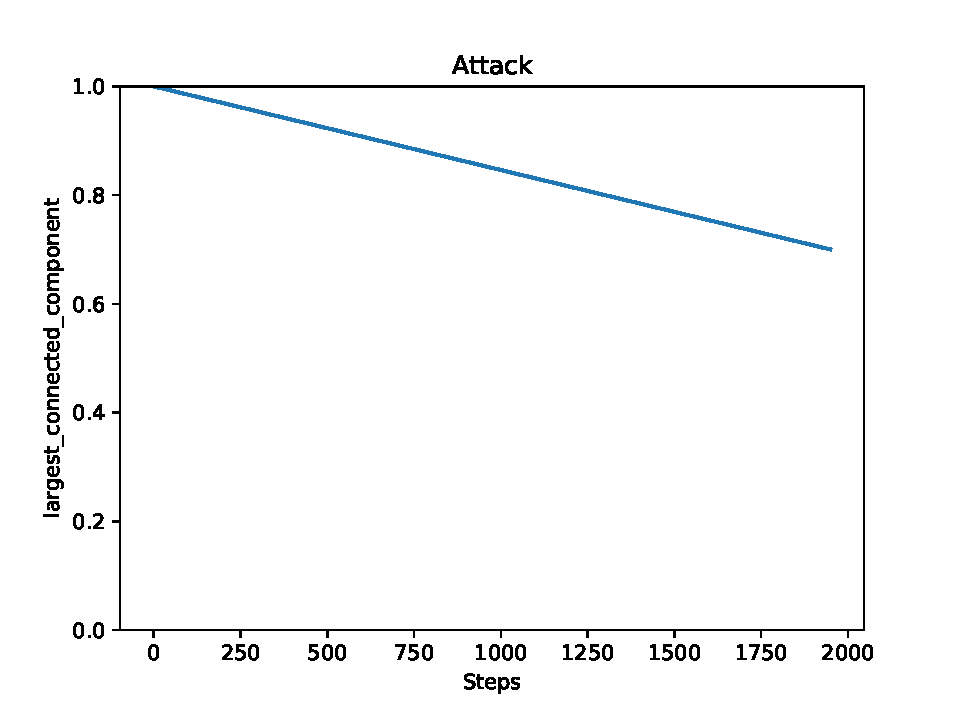
\includegraphics[width=\textwidth]{Images/plots_ib/ib_28.pdf}
		\caption{for $6500$ neurons}
		%\label{fig:y equals x}
	\end{subfigure}
	\hfill
	\begin{subfigure}[b]{0.45\textwidth}
		\centering
		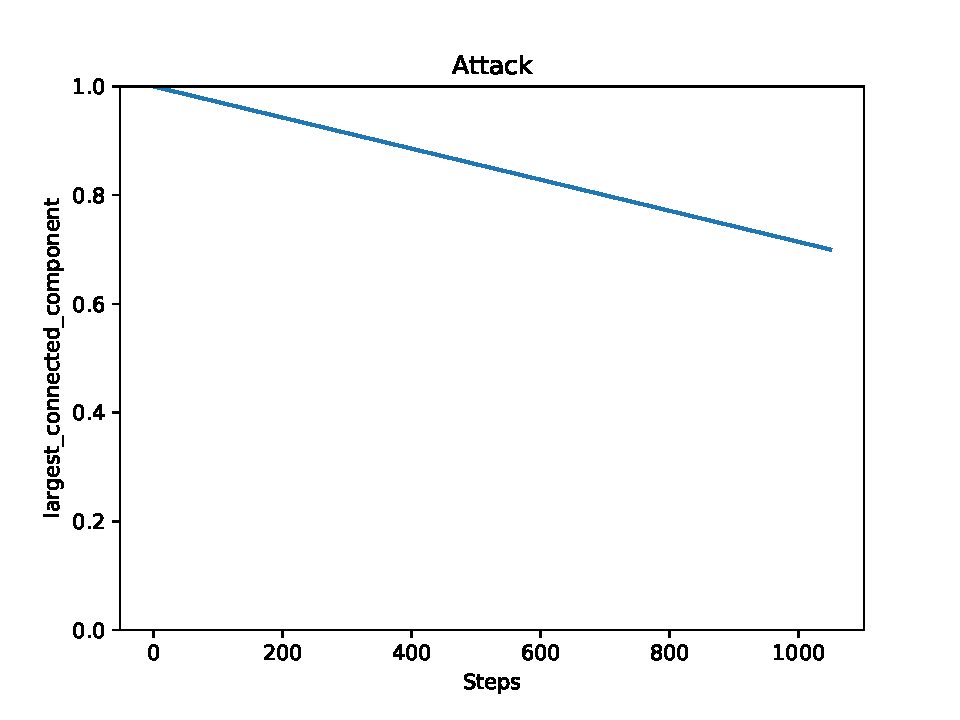
\includegraphics[width=\textwidth]{Images/plots_ib/ib_34.pdf}
		\caption{for $3500$ neurons}
		%\label{fig:three sin x}
	\end{subfigure}
	\\ \vspace{5mm}
	\begin{subfigure}[b]{0.45\textwidth}
		\centering
		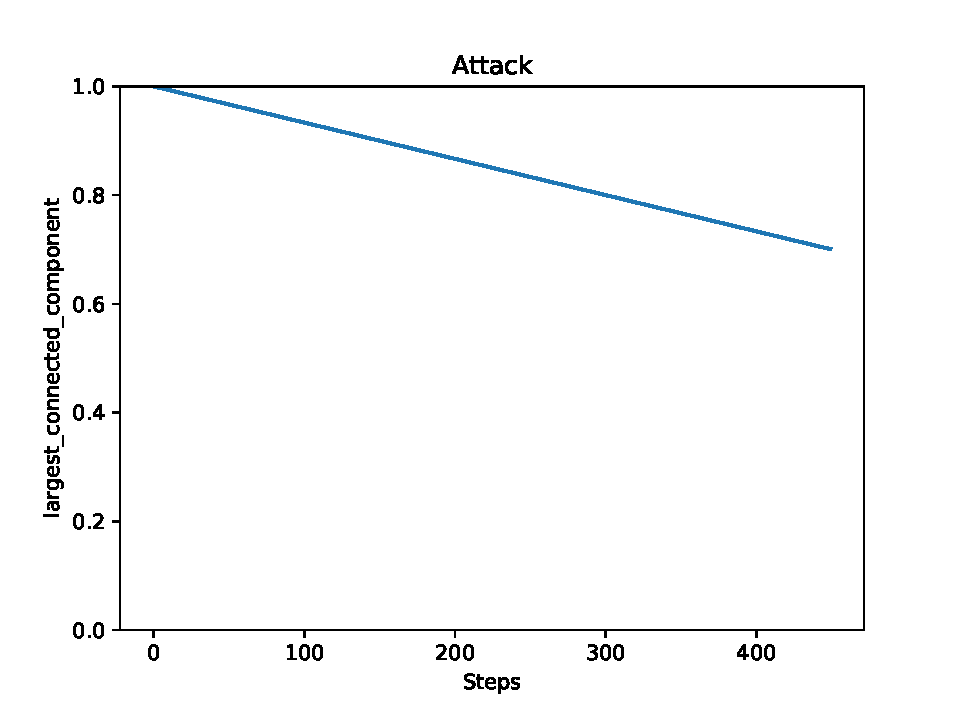
\includegraphics[width=\textwidth]{Images/plots_ib/ib_38.pdf}
		\caption{for $1500$ neurons}
		%\label{fig:y equals x}
	\end{subfigure}
	\hfill
	\begin{subfigure}[b]{0.45\textwidth}
		\centering
		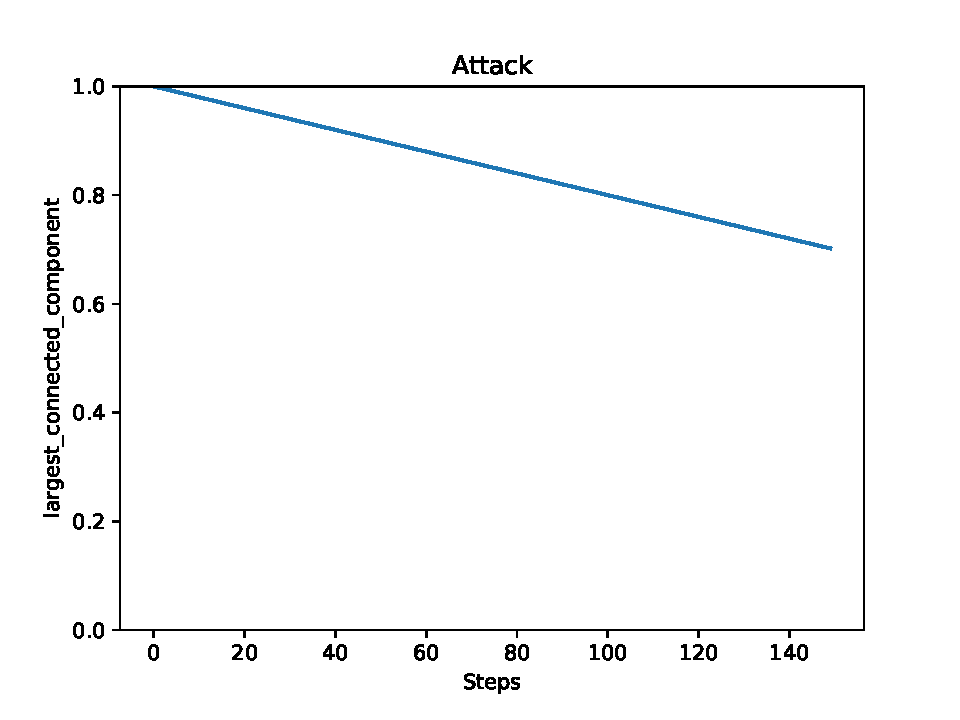
\includegraphics[width=\textwidth]{Images/plots_ib/ib_40.pdf}
		\caption{for $500$ neurons}
		%\label{fig:three sin x}
	\end{subfigure}
	\\ \vspace{5mm}
	
	
	\caption{Robustness of the network at various graining scales against removal of highest-betweenness nodes attack, using the largest connected component as measure.}
	\label{fig:ib_atk}
\end{figure}


% CASCADING ATTACK
\begin{figure}
	\centering
	\begin{subfigure}[b]{0.45\textwidth}
		\centering
		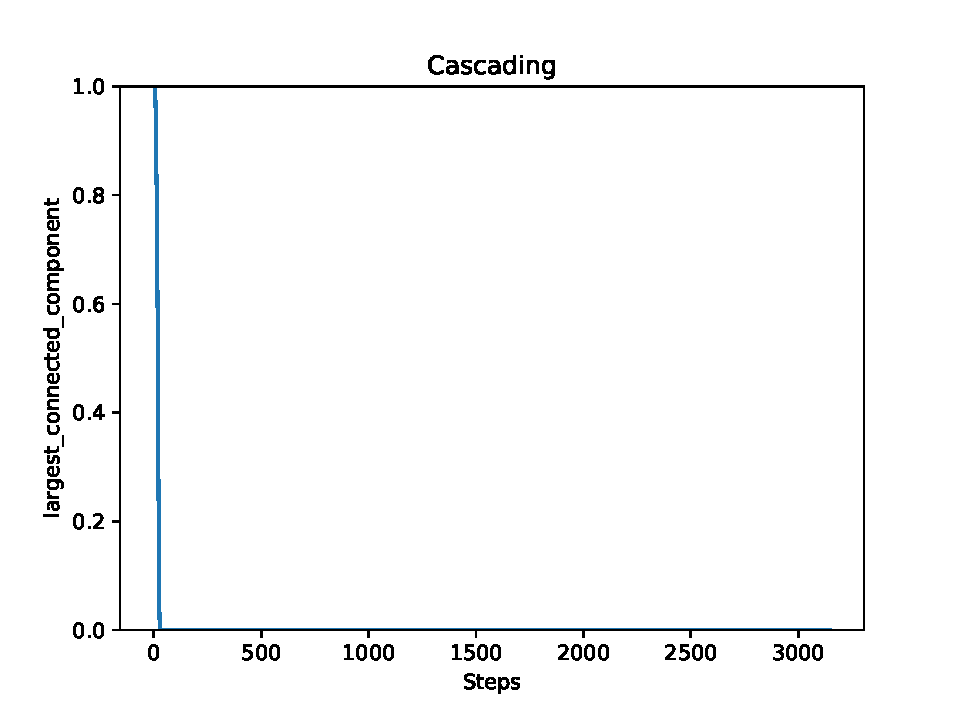
\includegraphics[width=\textwidth]{Images/plots_cascading/cascading_20.pdf}
		\caption{for $10500$ neurons}
		%\label{fig:y equals x}
	\end{subfigure}
	\hfill
	\begin{subfigure}[b]{0.45\textwidth}
		\centering
		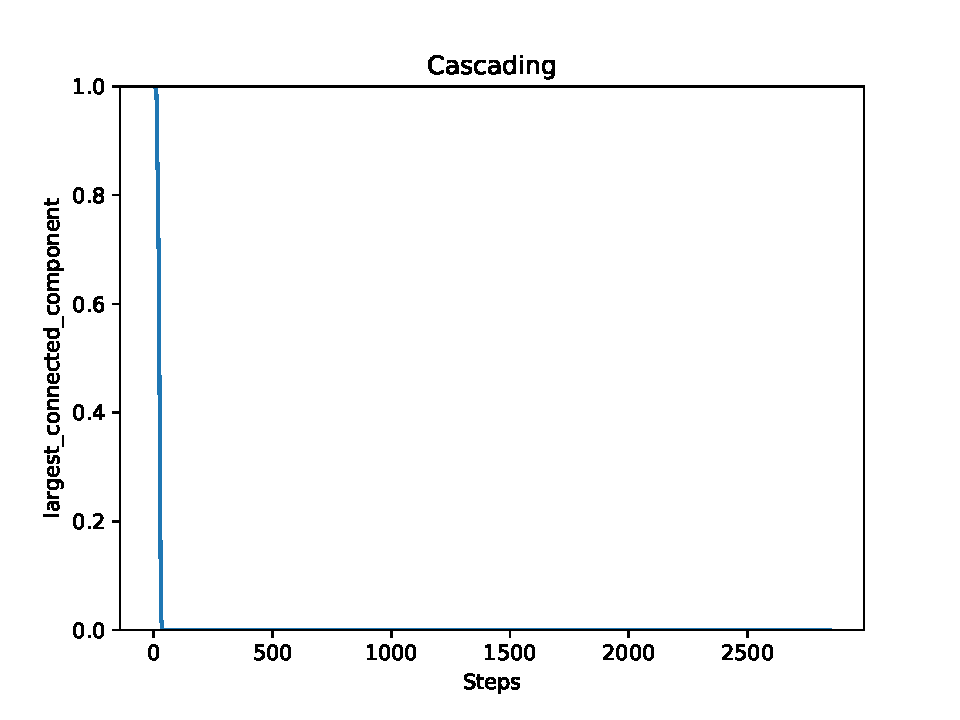
\includegraphics[width=\textwidth]{Images/plots_cascading/cascading_22.pdf}
		\caption{for $9500$ neurons}
		%\label{fig:three sin x}
	\end{subfigure}
	\\ \vspace{5mm}
	\begin{subfigure}[b]{0.45\textwidth}
		\centering
		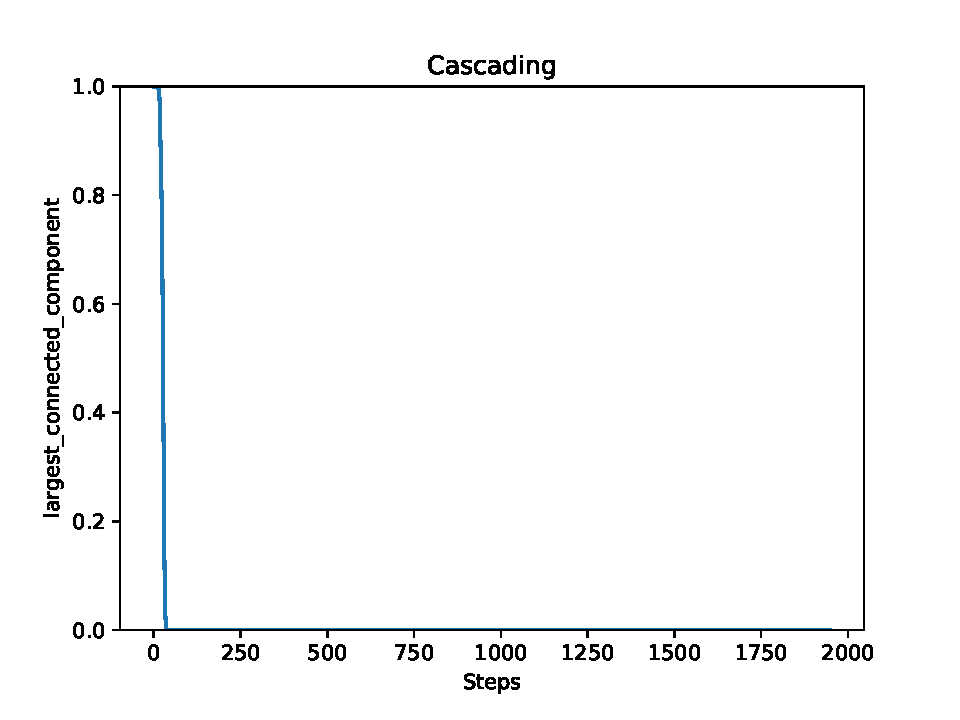
\includegraphics[width=\textwidth]{Images/plots_cascading/cascading_28.pdf}
		\caption{for $6500$ neurons}
		%\label{fig:y equals x}
	\end{subfigure}
	\hfill
	\begin{subfigure}[b]{0.45\textwidth}
		\centering
		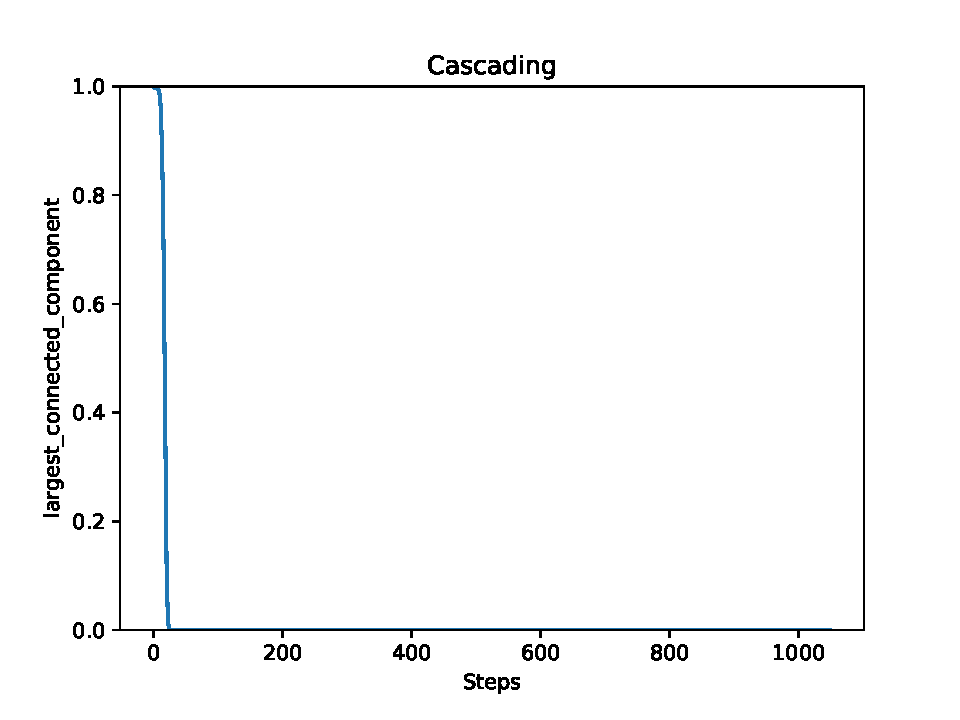
\includegraphics[width=\textwidth]{Images/plots_cascading/cascading_34.pdf}
		\caption{for $3500$ neurons}
		%\label{fig:three sin x}
	\end{subfigure}
	\\ \vspace{5mm}
	\begin{subfigure}[b]{0.45\textwidth}
		\centering
		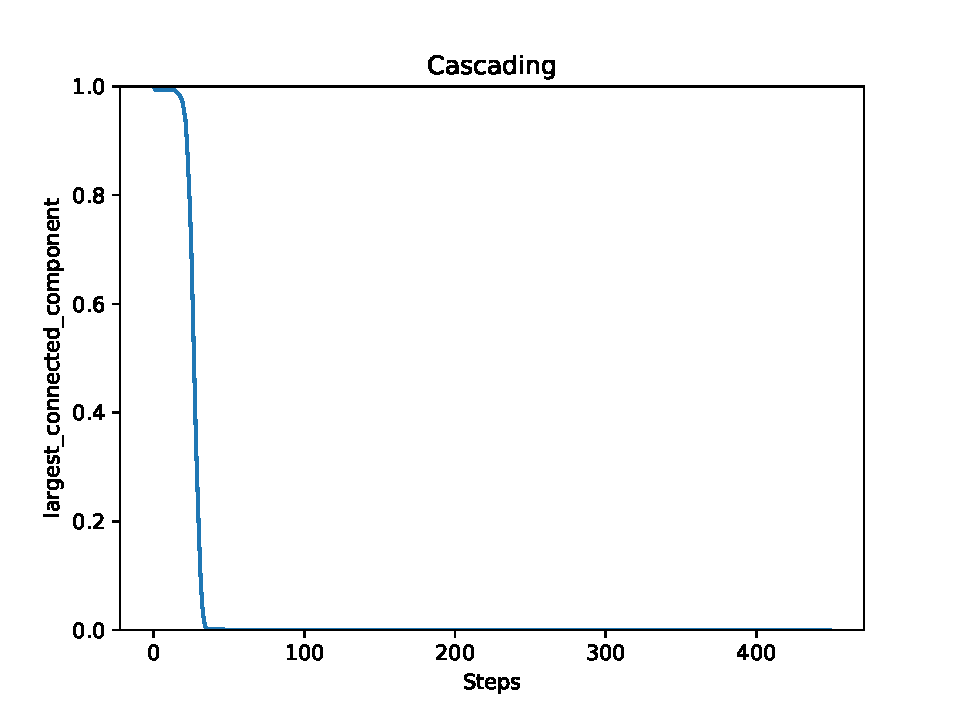
\includegraphics[width=\textwidth]{Images/plots_cascading/cascading_38.pdf}
		\caption{for $1500$ neurons}
		%\label{fig:y equals x}
	\end{subfigure}
	\hfill
	\begin{subfigure}[b]{0.45\textwidth}
		\centering
		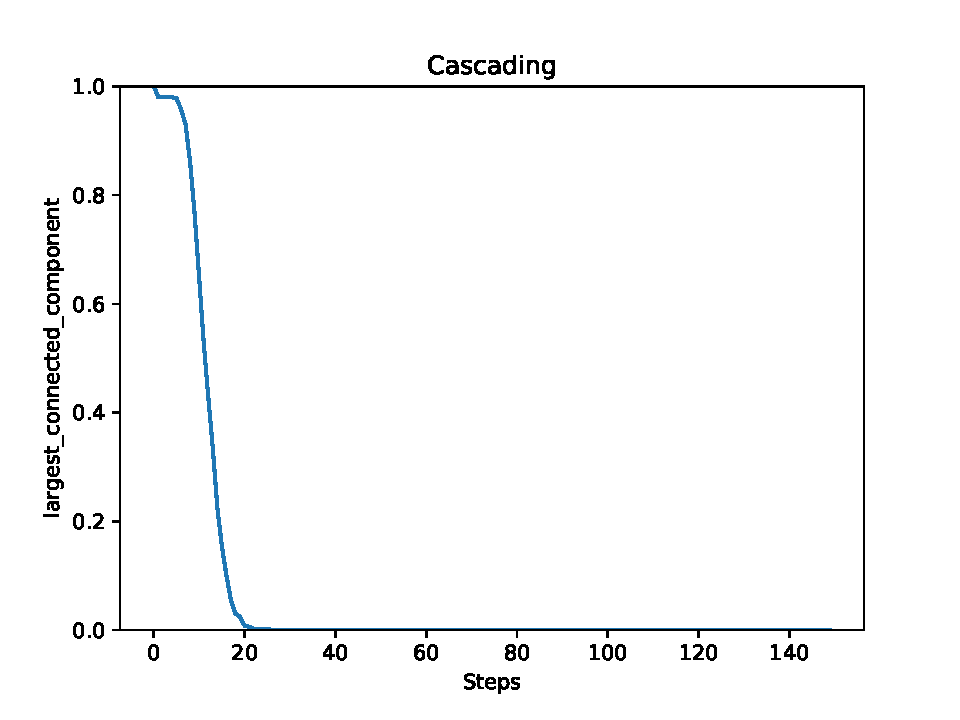
\includegraphics[width=\textwidth]{Images/plots_cascading/cascading_40.pdf}
		\caption{for $500$ neurons}
		%\label{fig:three sin x}
	\end{subfigure}
	\\ \vspace{5mm}
	
	
	\caption{Robustness of the network at various graining scales against removal of highest-betweenness nodes cascading attack, using the largest connected component as measure.}
	\label{fig:cascading_atk}
\end{figure}

% ADJACENCY MATRIX
\begin{figure}
    \centering
    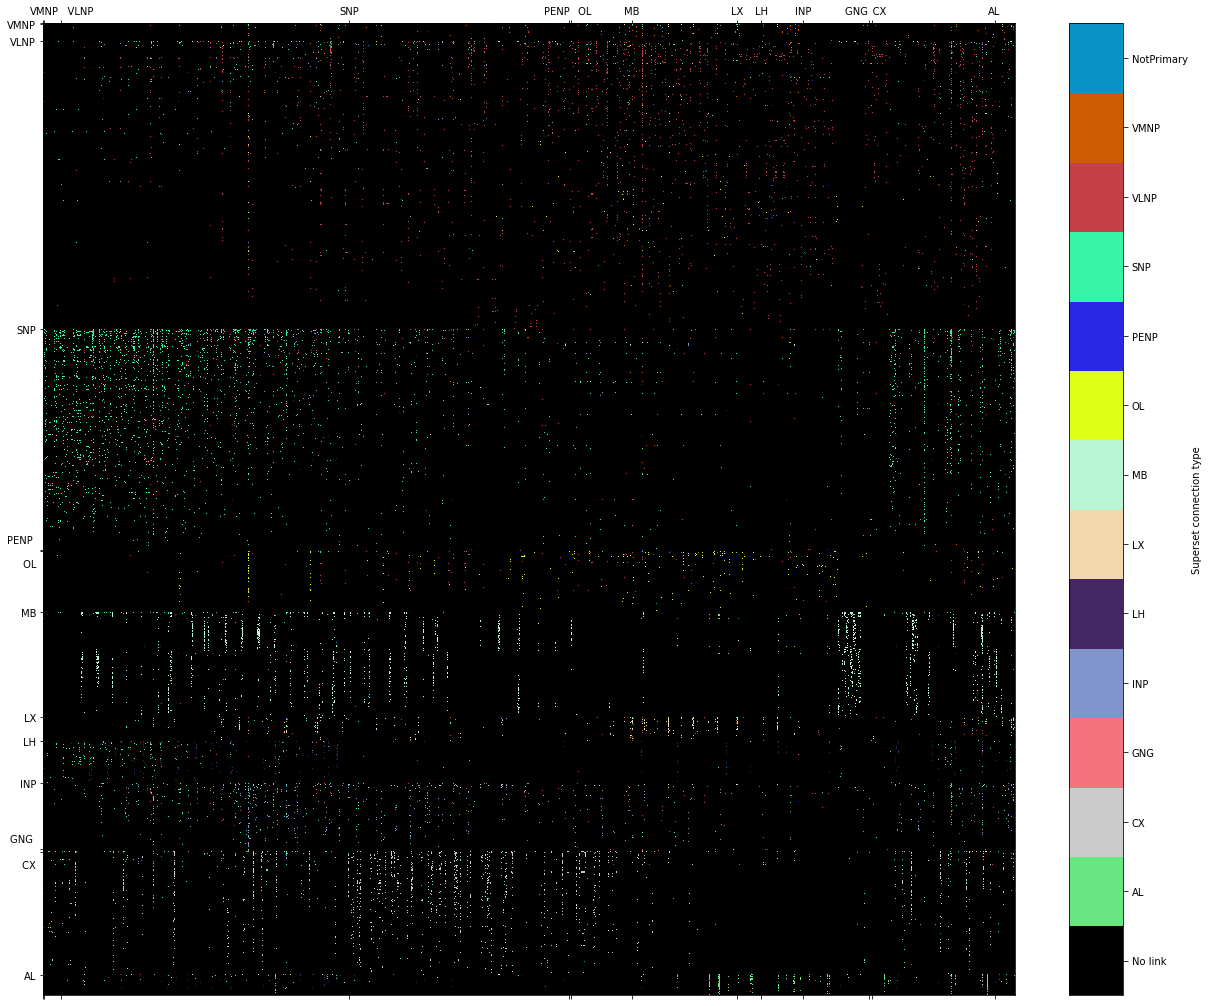
\includegraphics[width=\textwidth]{Images/Communities/Adj_matrix.png}
    \caption{Non weighted adjacency matrix of the full system. The neurons are ordered by community
    and then displayed in a decreasing degree order. In the y-axis the zone is, starting from its label, 
    up to the lower label. Similarly, for the x-axis the zone starts from the label and finishes to the next
    label to the right.}
    \label{fig:adj}
\end{figure}

% COMMUNITY EVOLUTION
\begin{figure}
    \centering
    \begin{subfigure}[t]{0.49\textwidth}
		\centering
		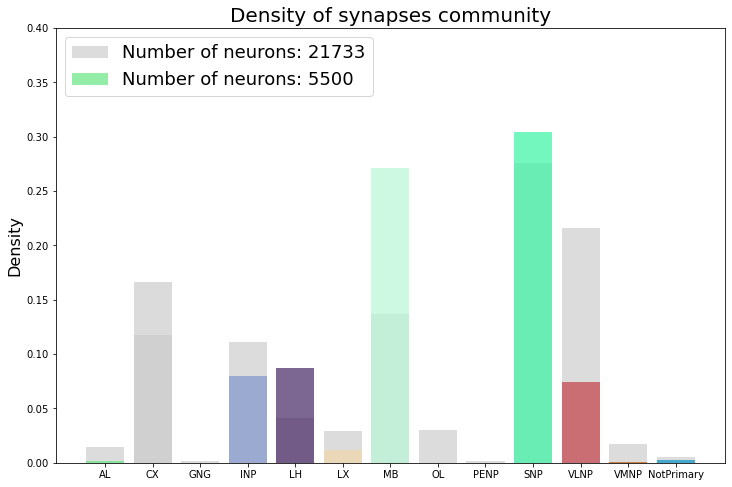
\includegraphics[width=\textwidth]{Images/Communities/Communities_after_graining.png}
		\caption{Density of the synapses communities before the coarse graining in gray, and 
		after the coarse graining with colors. We notice that the densities strongly vary in the 
		procedure.}
	\end{subfigure}
	\hfill
	\begin{subfigure}[t]{0.49\textwidth}
		\centering
		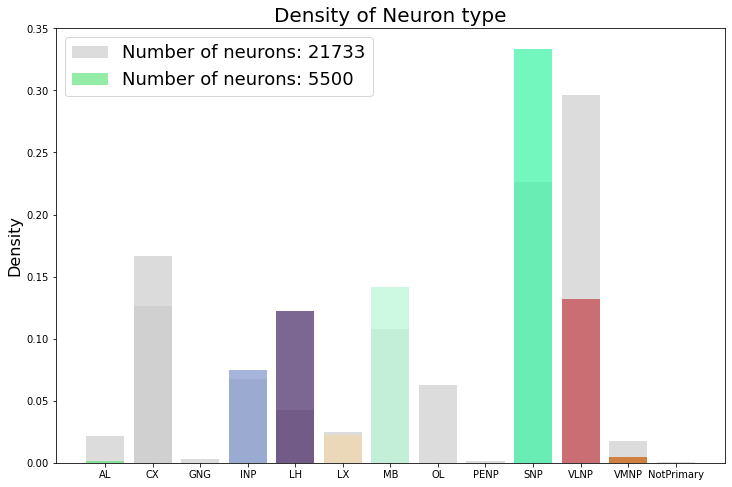
\includegraphics[width=\textwidth]{Images/Communities/density_neurons.png}
		\caption{Density of the synapses communities before the coarse graining in gray, and 
		after the coarse graining with colors, obtained using the methods described
		in the text. The distribution is similar,
		even if not the same, of the synapses distribution.}
	\end{subfigure}
	\caption{}
	\label{fig:com_evol}
\end{figure}

\begin{figure}
	\centering
	\begin{subfigure}[b]{0.49\textwidth}
		\centering
		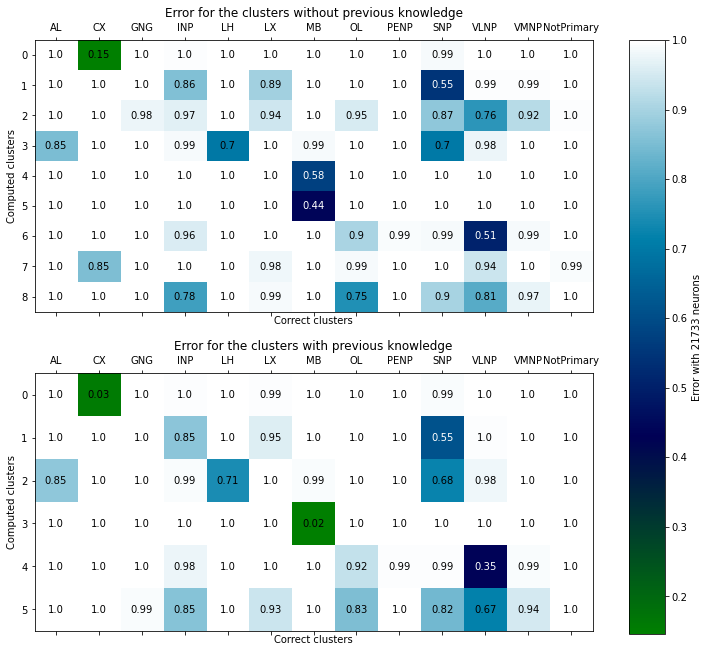
\includegraphics[width=\textwidth]{Images/Communities/Error_comm_21733.png}
		\caption{$21733$ neurons}
	\end{subfigure}
	\hfill
	\begin{subfigure}[b]{0.49\textwidth}
		\centering
		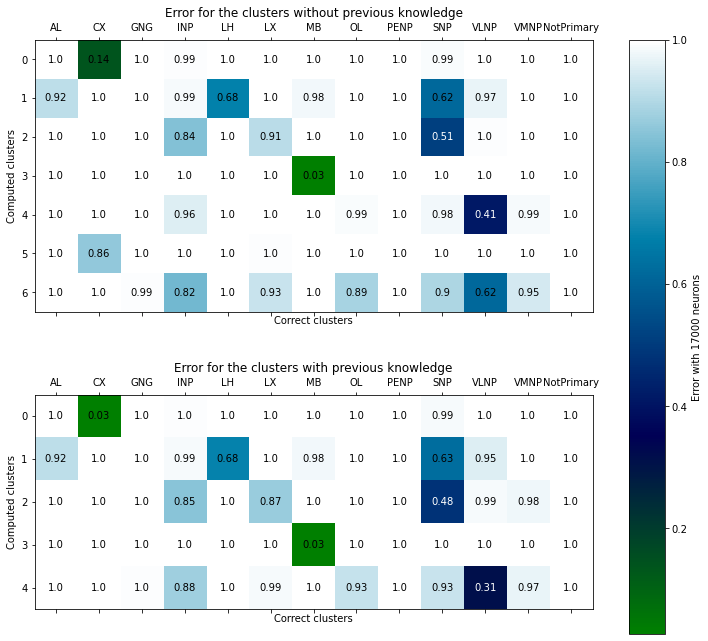
\includegraphics[width=\textwidth]{Images/Communities/Error_comm_17000.png}
		\caption{$17000$ neurons}
	\end{subfigure}
	\\ \vspace{5mm}
	\centering
	\begin{subfigure}[b]{0.49\textwidth}
		\centering
		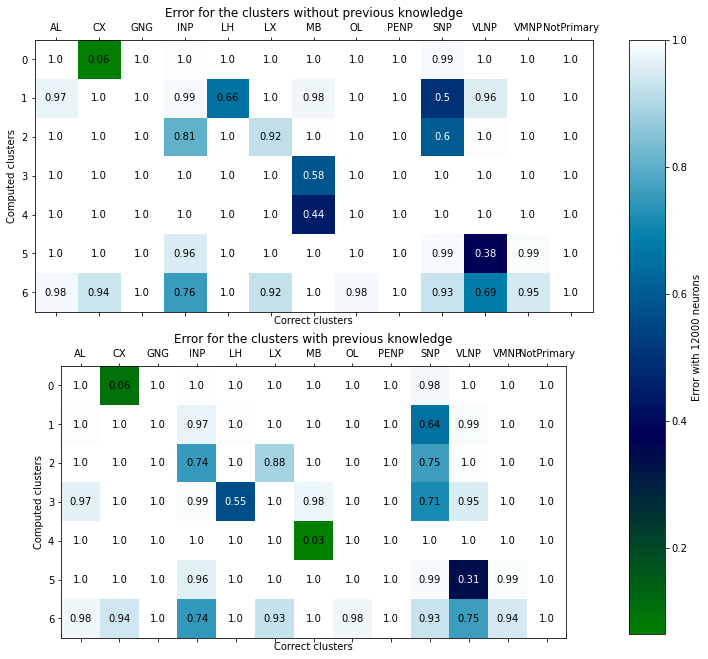
\includegraphics[width=\textwidth]{Images/Communities/Error_comm_12000.png}
		\caption{$12000$ neurons}
	\end{subfigure}
	\hfill
	\begin{subfigure}[b]{0.49\textwidth}
		\centering
		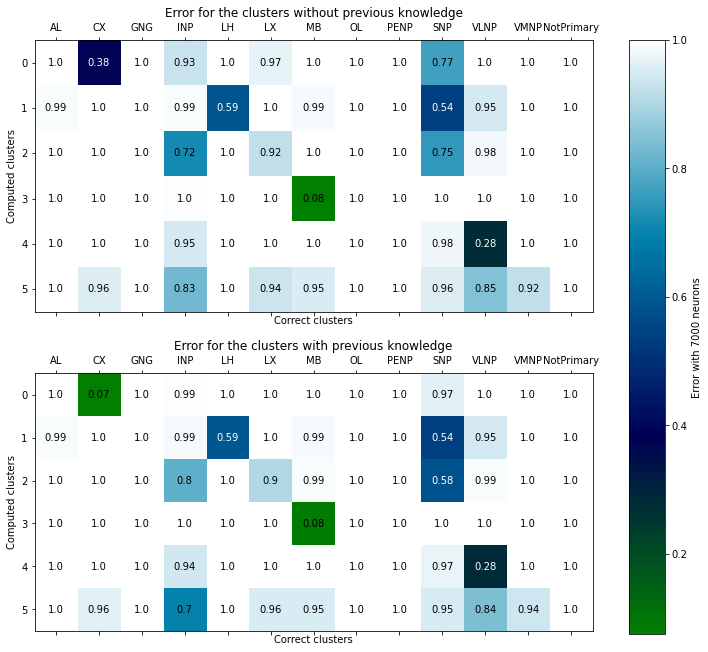
\includegraphics[width=\textwidth]{Images/Communities/Error_comm_7000.png}
		\caption{$7000$ neurons}
	\end{subfigure}
	\\ \vspace{5mm}
	\caption{Confusion matrices for different graining steps, starting forms
	both without previous knowledge and from the correct communities. On the x-axis
		we see the correct communities, while on the y-axis the communities detected
		by the Louvain algorithm. There is no preferred numbering on the communities.
		The error is defined as in Equation \ref{eq:com_er}.}
	\label{fig:cmaps}
\end{figure}